\chapter{Atomen en moleculen}\label{ch:g7:atoms-and-molecules}

Neem een druppel water en snijd hem in tweeën. Elke helft is nog steeds
water. Snijd een helft weer in tweeën, en nog eens, en nog eens. Kun je
eindeloos doorgaan, of kom je bij een stukje dat zo klein is dat je, als
je het nog één keer doorsnijdt, iets krijgt wat helemaal geen water meer
is? Rond 400~v.Chr. raadde de Griekse denker Democritus het antwoord:
materie bestaat uit piepkleine stukjes die niet te snijden zijn, die hij
\emph{\omterm{def:g7:atoms-and-molecules:atom}{atomen}} noemde, naar het Griekse woord voor ``ondeelbaar''. Het
kostte meer dan tweeduizend jaar, en het werk van de scheikundigen van
de negentiende eeuw, om van dat vermoeden wetenschap te maken. Dit
hoofdstuk beschrijft de stukjes --- de \omterm{def:g7:atoms-and-molecules:atom}{atomen} --- en hoe ze zich tot
\omterm{def:g7:atoms-and-molecules:molecule}{moleculen} groeperen.

\begin{recall}
Een \omterm{def:g6:pure-substances-and-mixtures:pure-substance}{zuivere stof}, zoals water of zuurstof, bestaat uit één enkele
\omterm{def:g6:pure-substances-and-mixtures:species}{chemische stof}; een \omterm{def:g6:pure-substances-and-mixtures:mixture}{mengsel}, zoals \omterm{def:g4:air-a-mixture-of-gases:air}{lucht}, bevat er meerdere
(\cref{ch:g6:pure-substances-and-mixtures}). \omterm{def:g4:air-a-mixture-of-gases:air}{Lucht} bestaat voor ongeveer
vier vijfde uit stikstof en voor een vijfde uit zuurstof
(\cref{ch:g4:air-a-mixture-of-gases}).
\end{recall}

\section{Atomen}

\begin{definition}[Atoom]\label{def:g7:atoms-and-molecules:atom}
Alle materie is opgebouwd uit uiterst kleine deeltjes die
\emph{atomen}\index{atoom} heten. In de natuur bestaan maar ongeveer
honderd verschillende soorten atomen, en elke stof --- water, \omterm{def:g4:air-a-mixture-of-gases:air}{lucht},
ijzer, suiker, ons eigen lichaam --- bestaat uit atomen van een paar van
die soorten.
\end{definition}

\begin{proposition}[Atomen zijn piepklein]\label{prop:g7:atoms-and-molecules:tiny}
% ledger: const:a0, earth:diameter (8 cm apple: 12756 km / 8 cm = 1.6 x 10^8;
% 0.1-0.15 nm x 1.6 x 10^8 = 1.7-2.4 cm, a small cherry)
Het kleinste \omterm{def:g7:atoms-and-molecules:atom}{atoom}, het waterstofatoom, is ongeveer een tienmiljoenste
millimeter breed; de andere zijn hoogstens een paar keer groter. Tien
miljoen waterstofatomen op een rij vormen een lijn van één millimeter.
Om het je voor te stellen: als een appel zo groot werd als de aarde, zou
elk van zijn \omterm{def:g7:atoms-and-molecules:atom}{atomen} ongeveer zo groot zijn als een kleine kers.
\end{proposition}

\begin{remark}[Gezien zonder gezien te worden]\label{rem:g7:atoms-and-molecules:seen}
Geen enkele lichtmicroscoop kan een \omterm{def:g7:atoms-and-molecules:atom}{atoom} laten zien: \omterm{def:g7:atoms-and-molecules:atom}{atomen} zijn veel
kleiner dan de golven van licht. Sinds de jaren tachtig maken speciale
microscopen, die een oppervlak aftasten met een uiterst fijne punt,
beelden waarop afzonderlijke \omterm{def:g7:atoms-and-molecules:atom}{atomen} als bobbeltjes te zien zijn.
\end{remark}

\begin{definition}[Symbool van een atoom]\label{def:g7:atoms-and-molecules:symbol}
Elke soort \omterm{def:g7:atoms-and-molecules:atom}{atoom} heeft een naam en een
\emph{symbool}\index{symbool van een atoom}: één hoofdletter, soms
gevolgd door één kleine letter. Het symbool is in elke taal hetzelfde.
\end{definition}

\begin{center}
\small
\begin{tabular}{llll|llll}
\hline
\omterm{def:g7:atoms-and-molecules:atom}{atoom} & \omterm{def:g7:atoms-and-molecules:symbol}{symbool} & & kleur in model & \omterm{def:g7:atoms-and-molecules:atom}{atoom} & \omterm{def:g7:atoms-and-molecules:symbol}{symbool} & & kleur in model \\
\hline
waterstof & \ce{H} & \tikz\node[aH]{}; & wit & natrium & \ce{Na} & \tikz\node[aNa]{}; & paars \\
koolstof & \ce{C} & \tikz\node[aC]{}; & zwart & zwavel & \ce{S} & \tikz\node[aS]{}; & geel \\
stikstof & \ce{N} & \tikz\node[aN]{}; & blauw & chloor & \ce{Cl} & \tikz\node[aCl]{}; & groen \\
zuurstof & \ce{O} & \tikz\node[aO]{}; & rood & ijzer, koper & \ce{Fe}, \ce{Cu} & & --- \\
\hline
\end{tabular}
\end{center}

\begin{remark}[Waar de symbolen vandaan komen]\label{rem:g7:atoms-and-molecules:latin}
De meeste symbolen zijn de beginletters van een oude, Latijnse naam:
\ce{H} van hydrogenium (waterstof), \ce{C} van carbonium (koolstof),
\ce{O} van oxygenium (zuurstof), \ce{Na} van \emph{natrium}, \ce{Fe} van
\emph{ferrum} (ijzer), \ce{Cu} van \emph{cuprum} (koper). De tweede
letter is altijd klein: \ce{Co} is het kobaltatoom, terwijl CO, met een
hoofdletter O, iets heel anders is.
\end{remark}

\begin{history}[De atomen van Dalton, 1808]
In 1808 publiceerde de scheikundige John Dalton een tabel van de \omterm{def:g7:atoms-and-molecules:atom}{atomen}
die toen bekend waren, elk getekend als een cirkeltje met een eigen
teken. Hij was de eerste die zei dat elk \omterm{def:g7:atoms-and-molecules:atom}{atoom} van één soort hetzelfde
gewicht heeft, en dat scheikundigen die gewichten konden vergelijken.
Maar hij dacht ook dat water uit één waterstofatoom en één zuurstofatoom
bestond; het duurde nog vijftig jaar voordat scheikundigen het erover
eens waren dat een watermolecuul \emph{twee} waterstofatomen bevat.
\end{history}

\begin{omfigure}
\begin{minipage}[b]{0.3\linewidth}\centering
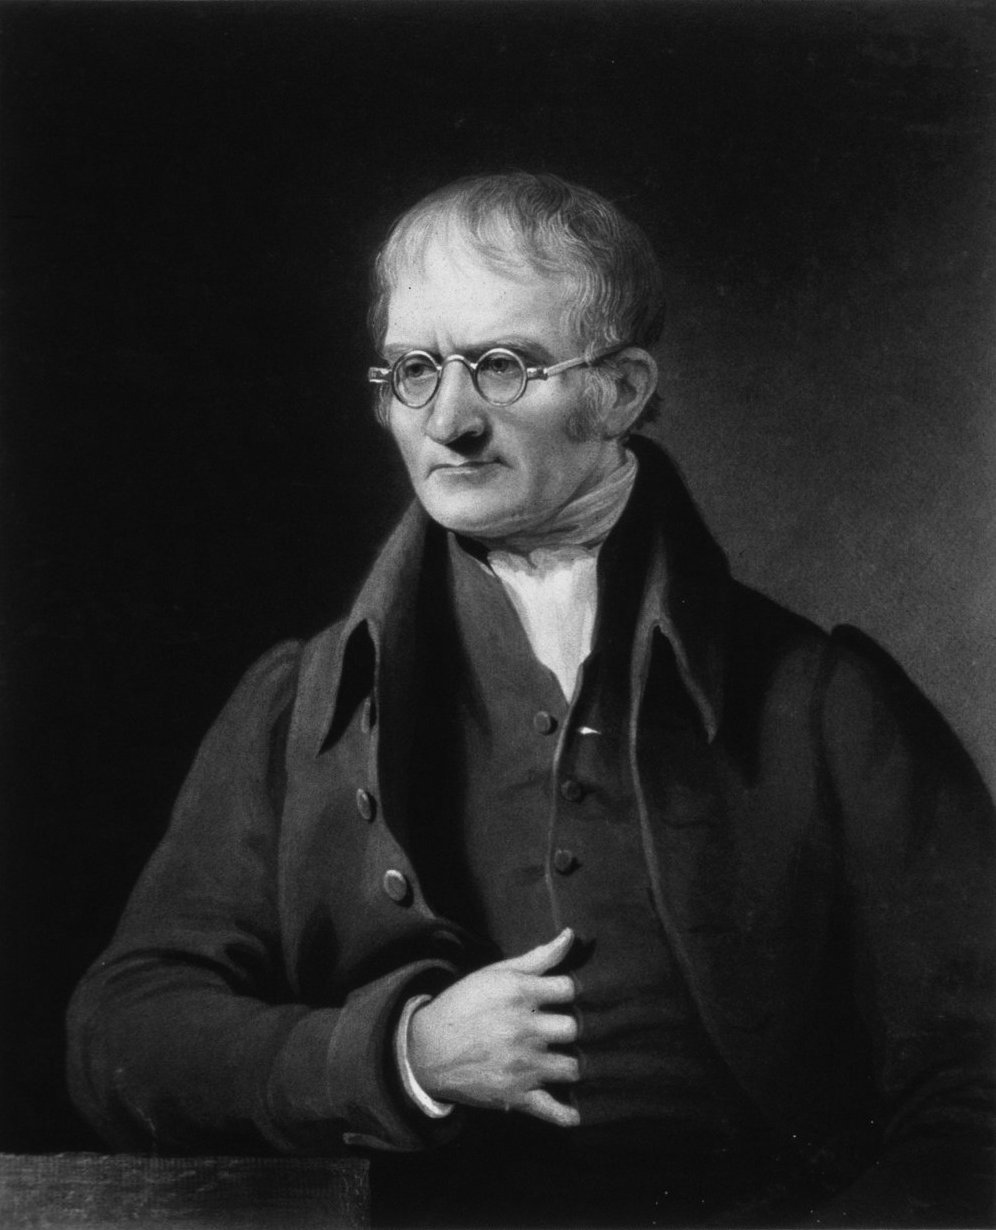
\includegraphics[width=\linewidth]{images/book1/dalton.jpg}

{\small John Dalton (1766--1844).}
\end{minipage}\hfill
\begin{minipage}[b]{0.66\linewidth}\centering
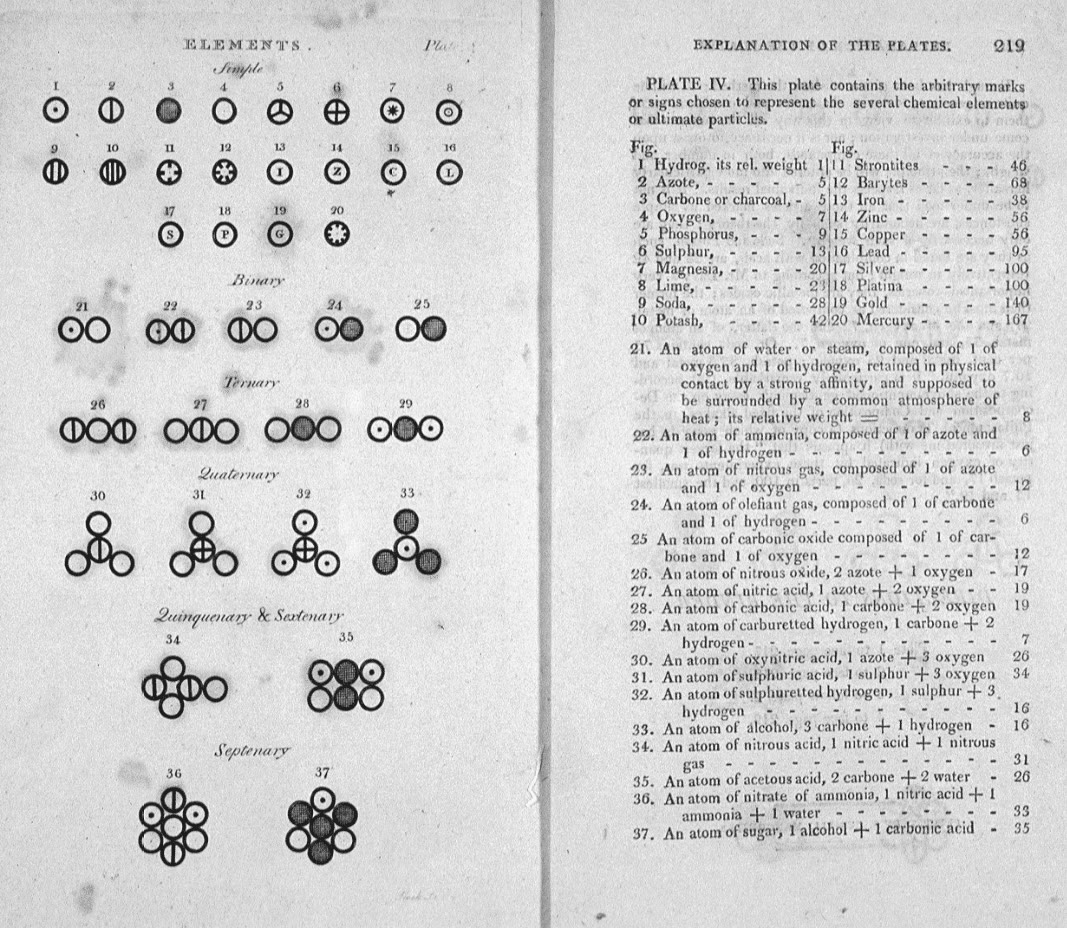
\includegraphics[width=\linewidth]{images/book1/dalton-symbols.jpg}

{\small De tabel van Dalton uit 1808: zijn water, teken 21, is één
cirkel waterstof naast één cirkel zuurstof.}
\end{minipage}
\end{omfigure}

\section{Moleculen}

\begin{definition}[Molecuul]\label{def:g7:atoms-and-molecules:molecule}
Een \emph{molecuul}\index{molecuul} is een groep \omterm{def:g7:atoms-and-molecules:atom}{atomen} die stevig aan
elkaar vastzitten. Een molecuul is het kleinste stukje van een stof dat
nog die stof is: een watermolecuul is de kleinst mogelijke hoeveelheid
water.
\end{definition}

\begin{example}[Zeven moleculen]\label{ex:g7:atoms-and-molecules:seven}
\begin{itemize}
  \item \emph{waterstof}: twee waterstofatomen;
  \item \emph{zuurstof}, dat we inademen: twee zuurstofatomen;
  \item \emph{stikstof}, vier vijfde van de \omterm{def:g4:air-a-mixture-of-gases:air}{lucht}: twee
        stikstofatomen;
  \item \emph{water}: twee waterstofatomen en één zuurstofatoom;
  \item \emph{koolstofdioxide}, dat we uitademen: één koolstofatoom en
        twee zuurstofatomen;
  \item \emph{methaan}, het hoofdbestanddeel van het aardgas dat in
        gasfornuizen verbrandt: één koolstofatoom en vier
        waterstofatomen;
  \item \emph{distikstofoxide}, een verdovend gas (lachgas):
        twee stikstofatomen en één zuurstofatoom.
\end{itemize}
\end{example}

\begin{omfigure}
\begin{tikzpicture}[font=\small]
  % hydrogen
  \begin{scope}[xshift=0cm]
    \node[aH] (a) at (-0.25,0) {}; \node[aH] (b) at (0.25,0) {};
    \begin{scope}[on background layer]\draw[bond] (a.center) -- (b.center);\end{scope}
    \node at (0,-1.05) {waterstof};
  \end{scope}
  % oxygen
  \begin{scope}[xshift=2.6cm]
    \node[aO] (a) at (-0.33,0) {}; \node[aO] (b) at (0.33,0) {};
    \begin{scope}[on background layer]
      \draw[bond, line width=1.1pt] ([yshift=1.6pt]a.center) -- ([yshift=1.6pt]b.center);
      \draw[bond, line width=1.1pt] ([yshift=-1.6pt]a.center) -- ([yshift=-1.6pt]b.center);
    \end{scope}
    \node at (0,-1.05) {zuurstof};
  \end{scope}
  % nitrogen
  \begin{scope}[xshift=5.2cm]
    \node[aN] (a) at (-0.33,0) {}; \node[aN] (b) at (0.33,0) {};
    \begin{scope}[on background layer]
      \foreach \d in {-2.4,0,2.4}
        \draw[bond, line width=0.9pt] ([yshift=\d pt]a.center) -- ([yshift=\d pt]b.center);
    \end{scope}
    \node at (0,-1.05) {stikstof};
  \end{scope}
  % water
  \begin{scope}[xshift=7.8cm, yshift=0.2cm]
    \node[aO] (o) at (0,0) {};
    \node[aH] (h1) at (-0.62,-0.48) {}; \node[aH] (h2) at (0.62,-0.48) {};
    \begin{scope}[on background layer]
      \draw[bond] (o.center) -- (h1.center); \draw[bond] (o.center) -- (h2.center);
    \end{scope}
    \node at (0,-1.25) {water};
  \end{scope}
  % carbon dioxide
  \begin{scope}[xshift=0.9cm, yshift=-2.7cm]
    \node[aO] (a) at (-0.85,0) {}; \node[aC] (c) at (0,0) {}; \node[aO] (b) at (0.85,0) {};
    \begin{scope}[on background layer]
      \foreach \d in {-1.6,1.6} {
        \draw[bond, line width=1.1pt] ([yshift=\d pt]a.center) -- ([yshift=\d pt]c.center);
        \draw[bond, line width=1.1pt] ([yshift=\d pt]c.center) -- ([yshift=\d pt]b.center);}
    \end{scope}
    \node at (0,-1.05) {koolstofdioxide};
  \end{scope}
  % methane
  \begin{scope}[xshift=4.4cm, yshift=-2.6cm]
    \node[aC] (c) at (0,0) {};
    \node[aH] (h1) at (0,0.78) {};
    \node[aH] (h2) at (-0.74,-0.3) {};
    \node[aH] (h3) at (0.74,-0.3) {};
    \begin{scope}[on background layer]
      \draw[bond] (c.center) -- (h1.center); \draw[bond] (c.center) -- (h2.center);
      \draw[bond] (c.center) -- (h3.center);
    \end{scope}
    \draw[bond] (c.center) -- (0.22,-0.52);
    \node[aH] at (0.24,-0.58) {};
    \node at (0,-1.15) {methaan};
  \end{scope}
  % nitrous oxide
  \begin{scope}[xshift=7.8cm, yshift=-2.7cm]
    \node[aN] (a) at (-0.8,0) {}; \node[aN] (b) at (0,0) {}; \node[aO] (c) at (0.8,0) {};
    \begin{scope}[on background layer]
      \foreach \d in {-1.6,1.6} {
        \draw[bond, line width=1.1pt] ([yshift=\d pt]a.center) -- ([yshift=\d pt]b.center);
        \draw[bond, line width=1.1pt] ([yshift=\d pt]b.center) -- ([yshift=\d pt]c.center);}
    \end{scope}
    \node at (0,-1.05) {distikstofoxide};
  \end{scope}
\end{tikzpicture}

{\small Bal-en-staafmodellen van de zeven \omterm{def:g7:atoms-and-molecules:molecule}{moleculen} van
\cref{ex:g7:atoms-and-molecules:seven}. Elk staafje stelt een binding
tussen twee \omterm{def:g7:atoms-and-molecules:atom}{atomen} voor; waarom sommige \omterm{def:g7:atoms-and-molecules:atom}{atomen} twee of drie staafjes
delen, legt een later hoofdstuk uit.}
\end{omfigure}

\begin{proposition}[Moleculen van een zuivere stof en van een mengsel]\label{prop:g7:atoms-and-molecules:pure}
In een \omterm{def:g6:pure-substances-and-mixtures:pure-substance}{zuivere stof} die uit \omterm{def:g7:atoms-and-molecules:molecule}{moleculen} bestaat, zijn alle \omterm{def:g7:atoms-and-molecules:molecule}{moleculen}
gelijk: zuiver water bevat alleen watermoleculen. Een \omterm{def:g6:pure-substances-and-mixtures:mixture}{mengsel} bevat
\omterm{def:g7:atoms-and-molecules:molecule}{moleculen} van meerdere soorten: \omterm{def:g4:air-a-mixture-of-gases:air}{lucht} bestaat vooral uit
stikstofmoleculen en zuurstofmoleculen, ongeveer vier van stikstof op
één van zuurstof, met een paar argonatomen die los blijven, en heel
weinig \omterm{def:g7:atoms-and-molecules:molecule}{moleculen} koolstofdioxide.
\end{proposition}

\begin{omfigure}
\begin{tikzpicture}[font=\small,
    sN/.style={aN, minimum size=3.0mm}, sO/.style={aO, minimum size=2.9mm},
    sH/.style={aH, minimum size=2.1mm}, sAr/.style={om atom, ball color=cyan!60, minimum size=3.4mm}]
  % air
  \draw[omGlass, line width=0.6pt] (0,0) rectangle (3.4,3.4);
  \foreach \x/\y/\r in {0.5/0.6/20, 1.6/0.4/-30, 2.8/0.7/75, 0.6/1.7/110,
                        2.0/1.5/10, 2.9/2.0/-60, 0.9/2.8/40, 2.1/2.9/-15}
    \node[sN] at ($(\x,\y)+(\r:0.12)$) {} node[sN] at ($(\x,\y)+(\r+180:0.12)$) {};
  \foreach \x/\y/\r in {1.3/1.1/60, 1.6/2.3/-40}
    \node[sO] at ($(\x,\y)+(\r:0.12)$) {} node[sO] at ($(\x,\y)+(\r+180:0.12)$) {};
  \node[sAr] at (2.9,3.0) {};
  \node[anchor=north] at (1.7,-0.1) {\textbf{lucht}: een mengsel};
  % water
  \begin{scope}[xshift=5.2cm]
    \draw[omGlass, line width=0.6pt] (0,0) rectangle (3.4,3.4);
    \foreach \x in {0,1,2,3,4} \foreach \y in {0,1,2,3,4} {
      \pgfmathsetmacro{\ang}{mod(73*\x+41*\y,360)}
      \begin{scope}[shift={({0.36+0.67*\x},{0.4+0.66*\y})}, rotate=\ang]
        \node[sH] at (-0.16,-0.12) {}; \node[sH] at (0.16,-0.12) {};
        \node[sO] at (0,0) {};
      \end{scope}}
    \node[anchor=north] at (1.7,-0.1) {\textbf{water}: een zuivere stof};
  \end{scope}
\end{tikzpicture}

{\small Enorm ingezoomd. Links: in \omterm{def:g4:air-a-mixture-of-gases:air}{lucht} zijn er veel meer
stikstofmoleculen (blauw) dan zuurstofmoleculen (rood), en een
argonatoom (lichtblauw) reist alleen; de \omterm{def:g7:atoms-and-molecules:molecule}{moleculen} van een gas zitten
ver uit elkaar. Rechts: in vloeibaar water zijn de \omterm{def:g7:atoms-and-molecules:molecule}{moleculen} allemaal
gelijk en raken ze elkaar.}
\end{omfigure}

\section{Chemische formules}

\begin{definition}[Chemische formule]\label{def:g7:atoms-and-molecules:formula}
De \emph{chemische formule}\index{chemische formule} van een \omterm{def:g7:atoms-and-molecules:molecule}{molecuul}
geeft de symbolen van zijn \omterm{def:g7:atoms-and-molecules:atom}{atomen}, elk gevolgd door een klein getal dat
onder de regel geschreven wordt --- de \emph{index}\index{index} --- en
dat aangeeft hoeveel \omterm{def:g7:atoms-and-molecules:atom}{atomen} van die soort het \omterm{def:g7:atoms-and-molecules:molecule}{molecuul} bevat. Een index 1
schrijf je niet.
\end{definition}

\begin{example}[De zeven formules]\label{ex:g7:atoms-and-molecules:formulas}
De \omterm{def:g7:atoms-and-molecules:molecule}{moleculen} van \cref{ex:g7:atoms-and-molecules:seven} hebben deze
formules:
\begin{center}
\begin{tabular}{lcl}
\hline
\omterm{def:g7:atoms-and-molecules:molecule}{molecuul} & formule & \omterm{def:g7:atoms-and-molecules:atom}{atomen} \\
\hline
waterstof & \ce{H2} & 2 waterstof \\
zuurstof & \ce{O2} & 2 zuurstof \\
stikstof & \ce{N2} & 2 stikstof \\
water & \ce{H2O} & 2 waterstof, 1 zuurstof \\
koolstofdioxide & \ce{CO2} & 1 koolstof, 2 zuurstof \\
methaan & \ce{CH4} & 1 koolstof, 4 waterstof \\
distikstofoxide & \ce{N2O} & 2 stikstof, 1 zuurstof \\
\hline
\end{tabular}
\end{center}
\end{example}

\begin{method}[Een formule lezen]\label{met:g7:atoms-and-molecules:read}
Zo lees je de formule van een \omterm{def:g7:atoms-and-molecules:molecule}{molecuul}:
\begin{enumerate}
  \item verdeel haar in symbolen: elk \omterm{def:g7:atoms-and-molecules:symbol}{symbool} begint met een hoofdletter;
  \item lees na elk \omterm{def:g7:atoms-and-molecules:symbol}{symbool} de \omterm{def:g7:atoms-and-molecules:formula}{index} (geen \omterm{def:g7:atoms-and-molecules:formula}{index} betekent 1);
  \item tel de \omterm{def:g7:atoms-and-molecules:formula}{indices} op om het totale aantal \omterm{def:g7:atoms-and-molecules:atom}{atomen} te krijgen.
\end{enumerate}
Voor \ce{C2H6O} (ethanol, de alcohol in dranken): 2 koolstof, 6
waterstof, 1 zuurstof, in totaal 9 \omterm{def:g7:atoms-and-molecules:atom}{atomen}.
\end{method}

\begin{remark}[Een getal ervoor]\label{rem:g7:atoms-and-molecules:coefficient}
Een getal vóór een formule telt \omterm{def:g7:atoms-and-molecules:molecule}{moleculen}: \ce{3H2O} betekent drie
watermoleculen, die samen 6 waterstofatomen en 3 zuurstofatomen
bevatten. Verwar \ce{O2}, één \omterm{def:g7:atoms-and-molecules:molecule}{molecuul} uit twee zuurstofatomen, niet met
\ce{2O}, twee zuurstofatomen die niet aan elkaar vastzitten.
\end{remark}

\begin{example}[Methaan in de keuken]\label{ex:g7:atoms-and-molecules:methane}
Het aardgas van een gasfornuis is grotendeels methaan, \ce{CH4}. Elk van
zijn \omterm{def:g7:atoms-and-molecules:molecule}{moleculen} is één koolstofatoom met vier waterstofatomen eromheen.
Het gas is onzichtbaar en reukloos: de ``gaslucht'' is een stof die er
met opzet aan wordt toegevoegd, zodat je een lek opmerkt.
\end{example}

\begin{omfigure}
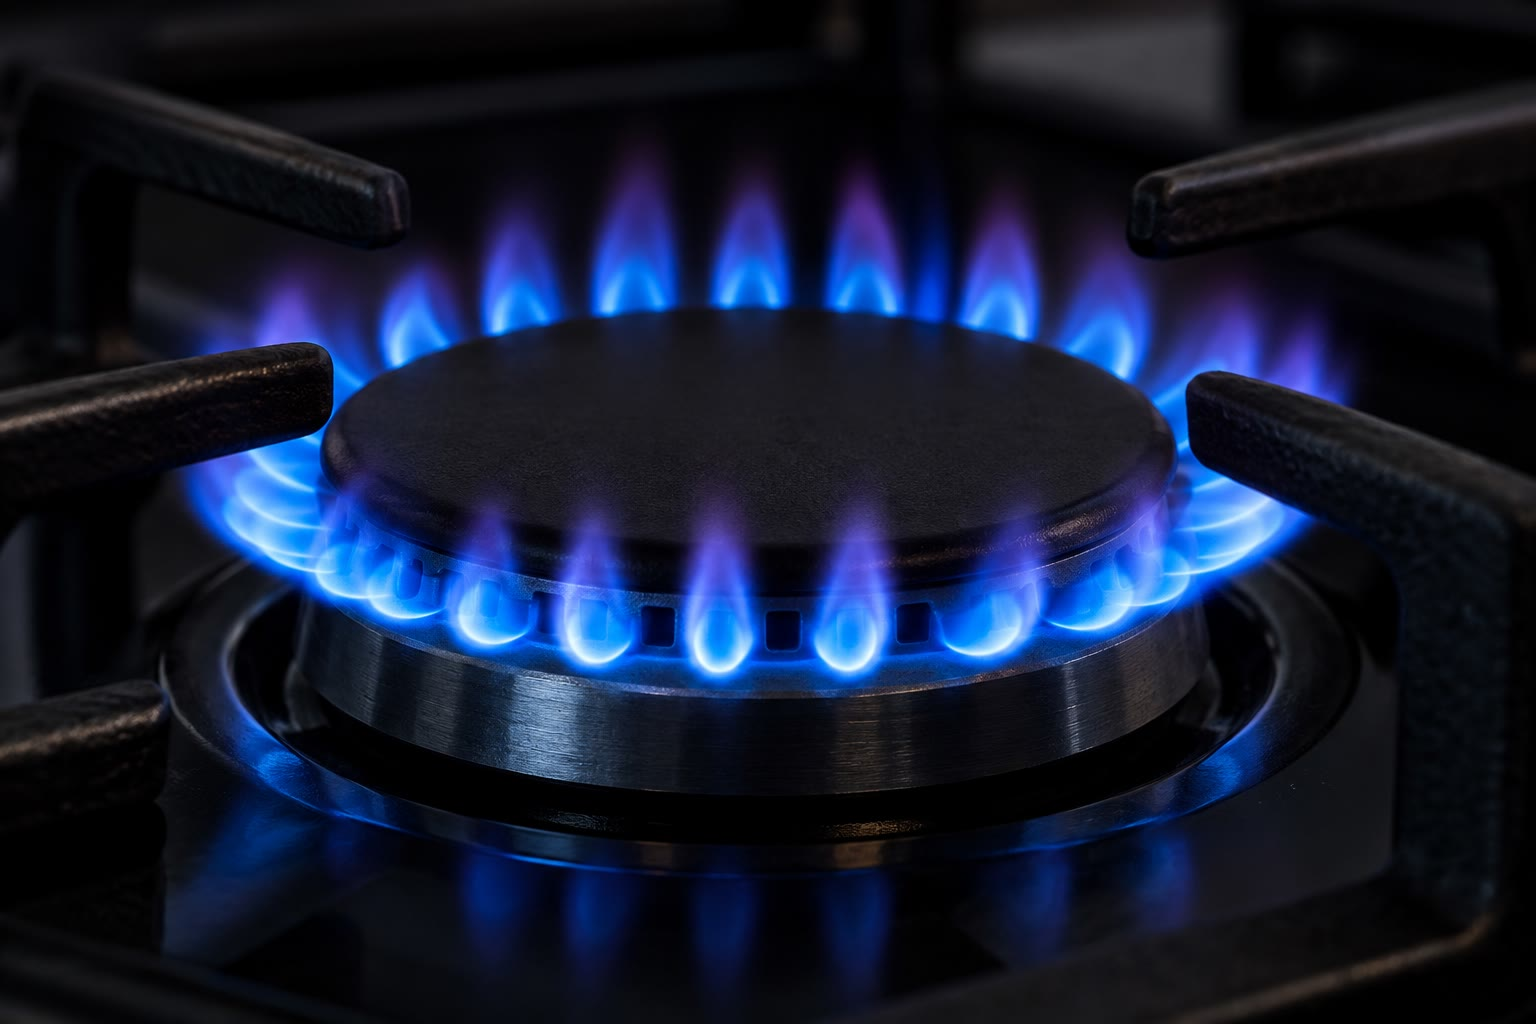
\includegraphics[width=0.5\linewidth]{images/book1/ai/g7-gas-flame.jpg}

{\small De blauwe vlam van een gasfornuis: het methaan van aardgas
verbrandt.}
\end{omfigure}

\section{Molecuulmodellen}

\begin{remark}[Modellen, en hun kleuren]\label{rem:g7:atoms-and-molecules:models}
Scheikundigen bouwen \emph{molecuulmodellen} met balletjes voor de
\omterm{def:g7:atoms-and-molecules:atom}{atomen} en staafjes voor de bindingen ertussen. De kleuren zijn een
afspraak die over de hele wereld gebruikt wordt --- koolstof zwart,
waterstof wit, zuurstof rood, stikstof blauw --- en niet de echte kleur
van \omterm{def:g7:atoms-and-molecules:atom}{atomen}: een los \omterm{def:g7:atoms-and-molecules:atom}{atoom} heeft helemaal geen kleur. Een model laat ook
de vorm van een \omterm{def:g7:atoms-and-molecules:molecule}{molecuul} zien, wat een formule niet doet: het
watermolecuul is gebogen, het koolstofdioxidemolecuul is recht.
\end{remark}

\begin{omfigure}
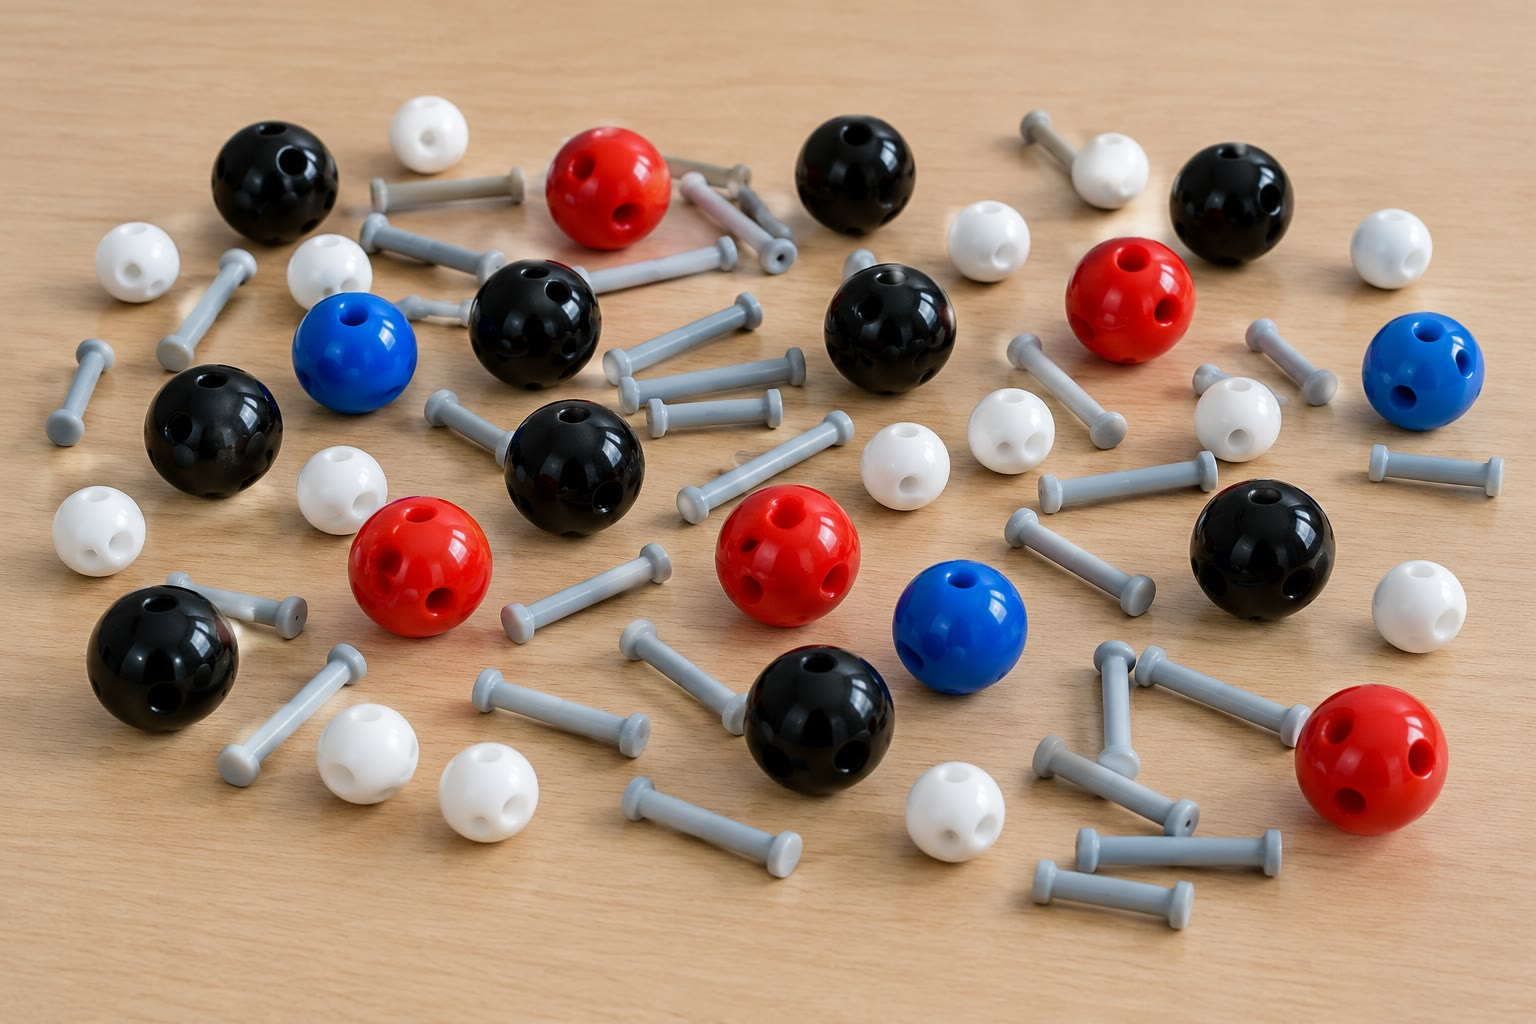
\includegraphics[width=0.5\linewidth]{images/book1/ai/g7-model-kit.jpg}

{\small Een molecuulbouwdoos: balletjes voor de \omterm{def:g7:atoms-and-molecules:atom}{atomen}, met gaatjes voor
de staafjes die de bindingen voorstellen.}
\end{omfigure}

\begin{method}[Van een model naar een formule]\label{met:g7:atoms-and-molecules:model}
Zo schrijf je de formule van een \omterm{def:g7:atoms-and-molecules:molecule}{molecuul} op uit zijn model:
\begin{enumerate}
  \item geef de \omterm{def:g7:atoms-and-molecules:atom}{atomen} een naam aan de hand van hun kleur;
  \item tel de balletjes van elke kleur;
  \item schrijf de symbolen op met de aantallen als \omterm{def:g7:atoms-and-molecules:formula}{index}, eerst
        koolstof, dan waterstof, dan de andere \omterm{def:g7:atoms-and-molecules:atom}{atomen} in alfabetische
        volgorde van hun symbolen.
\end{enumerate}
Een zwart balletje vast aan vier witte: één koolstof, vier waterstof,
\ce{CH4}.
\end{method}

\section{Oefeningen}

\begin{exercise}[$\star$]\label{exo:g7:atoms-and-molecules:1}
Wat is een \omterm{def:g7:atoms-and-molecules:atom}{atoom}? Wat is een \omterm{def:g7:atoms-and-molecules:molecule}{molecuul}?
\end{exercise}

\begin{exercise}[$\star$]\label{exo:g7:atoms-and-molecules:2}
Geef de symbolen van waterstof, koolstof, stikstof, zuurstof, natrium en
ijzer.
\end{exercise}

\begin{exercise}[$\star$]\label{exo:g7:atoms-and-molecules:3}
Hoeveel \omterm{def:g7:atoms-and-molecules:atom}{atomen} van elke soort zitten er in één \omterm{def:g7:atoms-and-molecules:molecule}{molecuul} koolstofdioxide,
\ce{CO2}? Hoeveel \omterm{def:g7:atoms-and-molecules:atom}{atomen} in totaal?
\end{exercise}

\begin{exercise}[$\star$]\label{exo:g7:atoms-and-molecules:4}
Geef de namen van de \omterm{def:g7:atoms-and-molecules:molecule}{moleculen} \ce{H2O}, \ce{O2}, \ce{CH4} en \ce{N2}.
\end{exercise}

\begin{exercise}[$\star$]\label{exo:g7:atoms-and-molecules:5}
Een \omterm{def:g7:atoms-and-molecules:molecule}{molecuul} stikstofdioxide, een bruin gas in vervuilde \omterm{def:g4:air-a-mixture-of-gases:air}{lucht}, bestaat
uit één stikstofatoom en twee zuurstofatomen. Schrijf de formule op.
\end{exercise}

\begin{exercise}[$\star\star$]\label{exo:g7:atoms-and-molecules:6}
Leg het verschil uit tussen \ce{O2} en \ce{2O}, en tussen \ce{CO} en
\ce{Co}.
\end{exercise}

\begin{exercise}[$\star\star$]\label{exo:g7:atoms-and-molecules:7}
Hoeveel waterstofatomen en hoeveel zuurstofatomen zitten er in
\ce{3H2O}? En in \ce{5O2}?
\end{exercise}

\begin{exercise}[$\star\star$]\label{exo:g7:atoms-and-molecules:8}
Een model bestaat uit één zwart balletje met twee rode balletjes eraan.
Geef de namen van de \omterm{def:g7:atoms-and-molecules:atom}{atomen}, schrijf de formule op en geef de naam van
het \omterm{def:g7:atoms-and-molecules:molecule}{molecuul}.
\end{exercise}

\begin{exercise}[$\star\star$]\label{exo:g7:atoms-and-molecules:9}
In de tabel van Dalton bestaat water uit één waterstofatoom en één
zuurstofatoom. Schrijf de formule op die Dalton in gedachten had, en zeg
hoeveel \omterm{def:g7:atoms-and-molecules:atom}{atomen} zijn watermolecuul tekortkomt.
\end{exercise}

\begin{exercise}[$\star\star$]\label{exo:g7:atoms-and-molecules:10}
Is zuiver water een \omterm{def:g6:pure-substances-and-mixtures:mixture}{mengsel}? En \omterm{def:g4:air-a-mixture-of-gases:air}{lucht}? Antwoord door de \omterm{def:g7:atoms-and-molecules:molecule}{moleculen} te
beschrijven die elk van beide bevat.
\end{exercise}

\begin{exercise}[$\star\star\star$]\label{exo:g7:atoms-and-molecules:11}
Een waterstofatoom is ongeveer een tienmiljoenste millimeter breed.
Hoeveel waterstofatomen naast elkaar vormen een lijn van \qty{1}{cm}?
En een lijn zo lang als een voetbalveld, \qty{100}{m}?
\end{exercise}

\begin{exercise}[$\star\star\star$]\label{exo:g7:atoms-and-molecules:12}
Glucose, de suiker die onze cellen voedt, heeft de formule
\ce{C6H12O6}. Hoeveel \omterm{def:g7:atoms-and-molecules:atom}{atomen} bevat één glucosemolecuul? Welk percentage
daarvan zijn waterstofatomen? Welk percentage koolstofatomen?
\end{exercise}

\section{Probleem: De atomen van een ademteug}

\begin{problem}[{Weekendprobleem --- de atomen in een teug lucht tellen,
voor en nadat die in onze longen is geweest}]
\label{pb:g7:atoms-and-molecules:1}
% ledger: air:N2, air:O2, air:Ar (78.08 / 20.95 / 0.93 rounded to 78 / 21 / 1),
% breath:O2, breath:CO2, breath:N2 (expired air: 16 / 4 / 78, water vapour removed)
Stikstof gaat onveranderd door de longen, en is daarom een goede
maatstaf. In droge \omterm{def:g4:air-a-mixture-of-gases:air}{lucht} zijn er op elke 78 stikstofmoleculen ongeveer
21 zuurstofmoleculen en 1 argonatoom: in totaal 100 deeltjes (\omterm{def:g7:atoms-and-molecules:molecule}{moleculen}
of losse \omterm{def:g7:atoms-and-molecules:atom}{atomen}). In uitgeademde \omterm{def:g4:air-a-mixture-of-gases:air}{lucht}, als de waterdamp eruit gehaald
is, gaan dezelfde 78 stikstofmoleculen samen met ongeveer 16
zuurstofmoleculen, 4 koolstofdioxidemoleculen en 1 argonatoom.

\medskip
\noindent\textbf{Deel I --- De \omterm{def:g4:air-a-mixture-of-gases:air}{lucht} die we inademen.}
\begin{enumerate}
  \item Schrijf de formules op van het stikstof-, het zuurstof- en het
        koolstofdioxidemolecuul, en geef van elk het aantal \omterm{def:g7:atoms-and-molecules:atom}{atomen}.
  \item Argon wordt in \omterm{def:g7:atoms-and-molecules:atom}{atomen} geteld, niet in \omterm{def:g7:atoms-and-molecules:molecule}{moleculen}. Wat zegt dat
        over argon?
  \item Hoeveel stikstofatomen zitten er in deze 100 deeltjes
        ingeademde \omterm{def:g4:air-a-mixture-of-gases:air}{lucht}? Hoeveel zuurstofatomen?
  \item Hoeveel \omterm{def:g7:atoms-and-molecules:atom}{atomen} zitten er in totaal in deze 100 deeltjes?
  \item Welk percentage van deze \omterm{def:g7:atoms-and-molecules:atom}{atomen} zijn stikstofatomen? Rond af op
        een geheel getal.
\end{enumerate}

\medskip
\noindent\textbf{Deel II --- De \omterm{def:g4:air-a-mixture-of-gases:air}{lucht} die we uitademen.}
\begin{enumerate}[resume]
  \item Hoeveel zuurstofatomen zitten er in de uitgeademde \omterm{def:g4:air-a-mixture-of-gases:air}{lucht} die bij
        dezelfde 78 stikstofmoleculen hoort, in zuurstofmoleculen? In
        koolstofdioxidemoleculen? In totaal?
  \item Vergelijk met vraag 3. Hoeveel zuurstofatomen ontbreken er? In
        welk \omterm{def:g7:atoms-and-molecules:molecule}{molecuul}, dat het lichaam maakt met de waterstof uit het
        voedsel en dat hier met de waterdamp verwijderd is, zijn ze
        terechtgekomen?
  \item Hoeveel koolstofatomen zitten er in de ingeademde \omterm{def:g4:air-a-mixture-of-gases:air}{lucht}? En in de
        uitgeademde \omterm{def:g4:air-a-mixture-of-gases:air}{lucht}?
  \item \omterm{def:g4:air-a-mixture-of-gases:air}{Lucht} brengt geen koolstofatomen in de longen. Waar kunnen de
        koolstofatomen van de adem vandaan komen? (Denk aan wat het
        lichaam gebruikt om te leven.)
  \item Hoeveel zuurstofmoleculen zijn er verdwenen, en hoeveel
        koolstofdioxidemoleculen zijn erbij gekomen?
\end{enumerate}

\medskip
\noindent\textbf{Deel III --- De telling.}
\begin{enumerate}[resume]
  \item Beschrijf het bal-en-staafmodel van elk van de vier soorten
        deeltjes in uitgeademde \omterm{def:g4:air-a-mixture-of-gases:air}{lucht}, met de kleuren van de balletjes
        (argon wordt getekend als één lichtblauw balletje).
  \item Hoeveel \omterm{def:g7:atoms-and-molecules:atom}{atomen} zitten er in totaal in de gedroogde uitgeademde
        \omterm{def:g4:air-a-mixture-of-gases:air}{lucht}? Hoeveel \omterm{def:g7:atoms-and-molecules:atom}{atomen} meer is dat dan in de ingeademde \omterm{def:g4:air-a-mixture-of-gases:air}{lucht}? Leg
        het verschil uit met de gewonnen koolstofatomen en de ontbrekende
        zuurstofatomen.
\end{enumerate}
\end{problem}
